This appendix provides information on the human data collection interface described in \S\ref{sec:data_collection}, which facilitates data collection from \texttt{GLEE} games played between humans and LLMs.

One of the main objectives of collecting data from language games is to compare the behavior of LLMs with human behavior in economic and strategic situations. To facilitate this comparison, we developed an interface that allows human players to play all the language games that can be defined using \texttt{GLEE}. The interface transforms the various prompts presented to LLMs into user-friendly screens for human participants, displaying the prompt and requesting them to send messages and make decisions.\footnote{Since human players are accustomed to being addressed by their first name (rather than as Alice or Bob), we asked them to enter their name at the beginning of the game and referred to them by their name throughout the game. The player's name was the only difference between the human player and the LLM-based player.} Through this interface, we enable human players to take on the role of one of the players while the other player is a pre-selected LLM. The interface is one of the contributions of this paper. Screenshots of the interface can be found in Appendix \ref{app:interface}.

The interface, developed using oTree~\parencite{CHEN201688}, enables integration with Amazon's crowdsourcing platform, mTurk,\footnote{\url{https://www.mturk.com/}.} through which we recruited 3,405 players who participated in various configurations against Gemini-1.5-flash. We chose Gemini-1.5-flash since it demonstrated strong performance compared to other LLMs and allowed comprehensive data collection due to its low usage cost. Since we aimed to collect multiple games from each configuration, we had to select a limited set of configurations for human participants to play. The process of selecting these sets is described in Appendix \ref{app:human_configs}. We collected human data from 195 different configurations: 78 of which were bargaining games, 60 of which were negotiation games, and 57 were persuasion games.

Each human player was allowed to play one game every 12 hours from each family of games. Human players were paid a base rate calculated at \$6 per hour, plus an average bonus of \$6 per hour. In total, we paid \$2,245 to all players for their participation in the games.
Bonuses were dependent on the configuration the human players played and their success in the game. The average bonus was known to players at the start of the game, aiming to encourage serious gameplay. To ensure players remained focused and made thoughtful decisions, we conducted two attention checks during the experiment, detailed in Appendix \ref{app:attention_test}. Players who failed in one of the attention checks were excluded from the dataset.
To reflect the real-world significance of the magnitude of product prices (the parameter M) in each family of games, we defined the bonus as dependent on M: in configurations where M = $10^2$, the average bonus was \$3 per hour; where M = $10^4$, the average bonus was \$6 per hour; and where M = $10^6$, the average bonus was \$9 per hour.



\subsection{Screenshots of the Data Collection Interface}
\label{app:interface}

\paragraph{General Application Structure}
The structure of the application and the games consists of fixed parts and parts that vary between different game families. Each game starts with a screen where the player enters their name, followed by an instruction screen (Figure \ref{fig:bargaining_intro} in bargaining, Figure \ref{fig:negotiation_intro} in negotiation, and Figure \ref{fig:persuasion_seller_intro} in persuasion). The instructions themselves can change depending on the type of game and the parameters of the game.
In the middle of the game’s rules on the instruction screen, there is a hidden prompt directing participants to enter a code word in the text box below. This test is designed to filter out unfocused participants.
If the player fails this test, they are directed to a screen informing them of their failure and will not participate in the game. Otherwise, the game begins. In each round, both the human player and the LLM player perform an action, with the order depending on the game and configuration. An action could involve sending an offer to the other player
(Figure \ref{fig:bargaining_proposer} in bargaining games, Figure \ref{fig:negotiation_proposer} in negotiation games and
Figure \ref{fig:persuasion_proposer} in Persuasion games)
or responding to the other player's offer (for instance, Figure \ref{fig:bargaining_receiver} in bargaining games, Figure \ref{fig:negotiation_receiver} in negotiation games and
Figure \ref{fig:persuasion_receiver} in persuasion games). After both players have completed their actions, the human player is taken to a response screen (Figure \ref{fig:bargaining_response}), where he sees the decision of the LLM player. Afterward, if the game is still not over, the human player continues for another round. Once the game is finished, the player is taken to a quiz screen where they must answer a question related to the technical details of the game (Figure \ref{fig:fina_quiz}). If the human answer correctly, they are directed to the final screen (Figure \ref{fig:game_over}), where they receive a code to enter on the mTurk website. If the player fails the final quiz, they do not receive a completion code and are taken to a screen that informs them of their failure in the quiz. In this case, we erase the game from our database.

\subsubsection{Bargaining Games Screenshots}

\begin{figure}[H]
\centering
\fbox{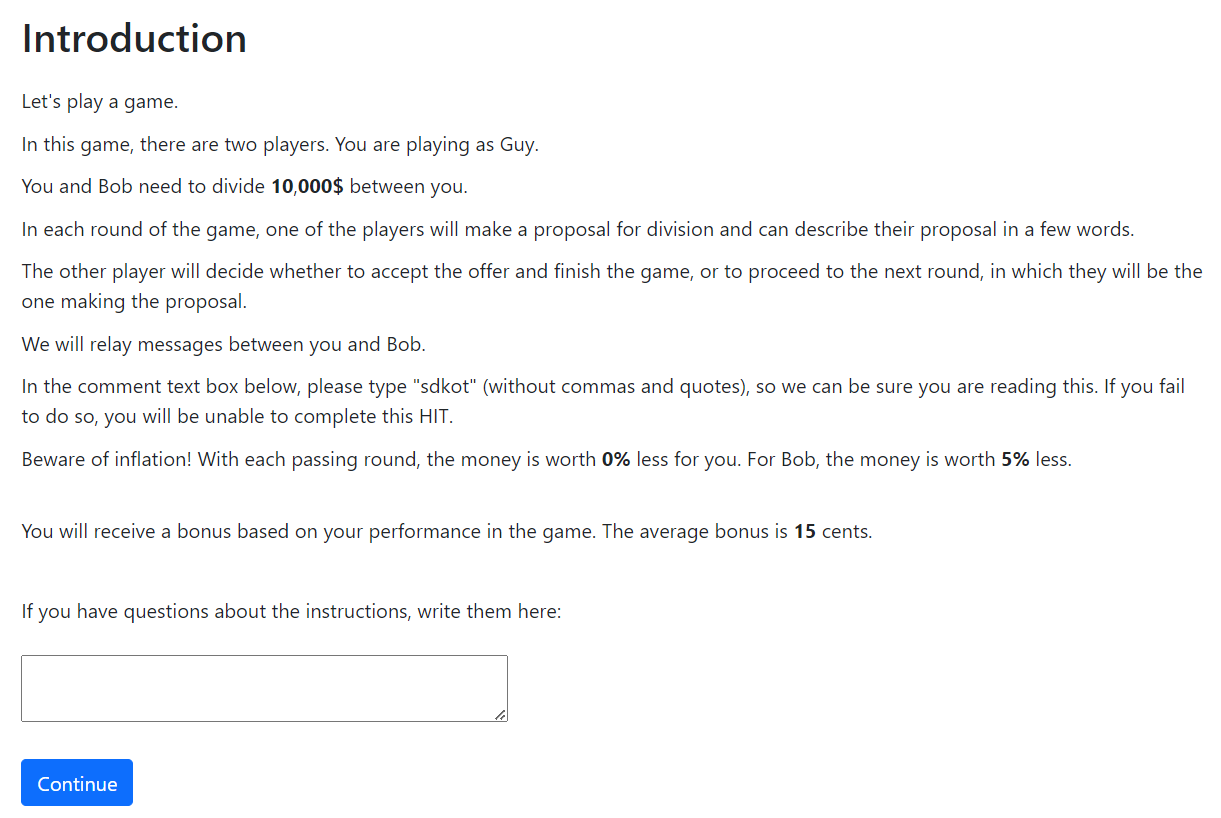
\includegraphics[width=0.9\textwidth,height=\textheight,keepaspectratio]{screenshots/bargaining_intro.png}}
\caption{An example of an instruction screen shown to a human player at the start of a bargaining game.}
\label{fig:bargaining_intro}
\end{figure}

\begin{figure}[H]
\centering
\fbox{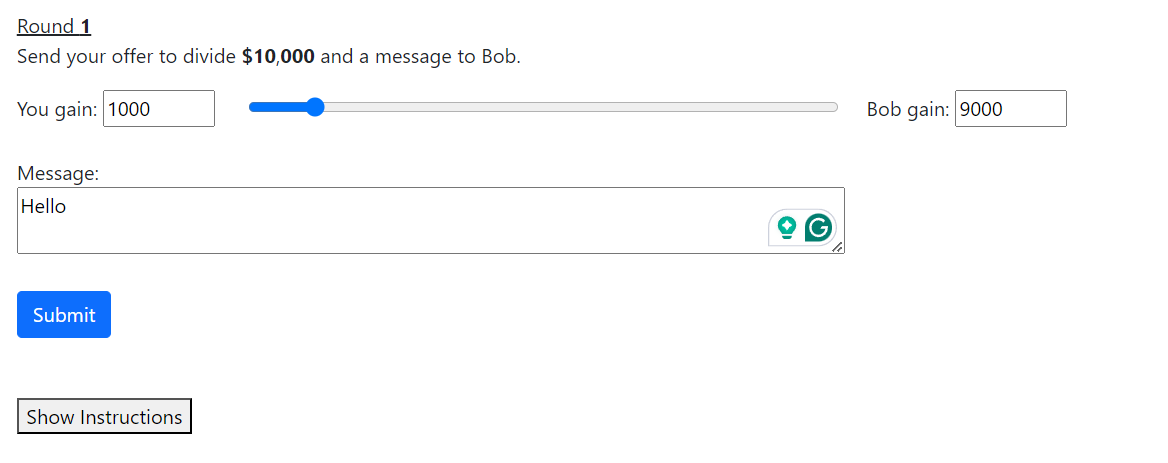
\includegraphics[width=0.9\textwidth,height=\textheight,keepaspectratio]{screenshots/bargaining_proposer.png}}
\caption{An example of a proposition screen shown to a human player during his first turn in a bargaining game.}
\label{fig:bargaining_proposer}
\end{figure}

\begin{figure}[H]
\centering
\fbox{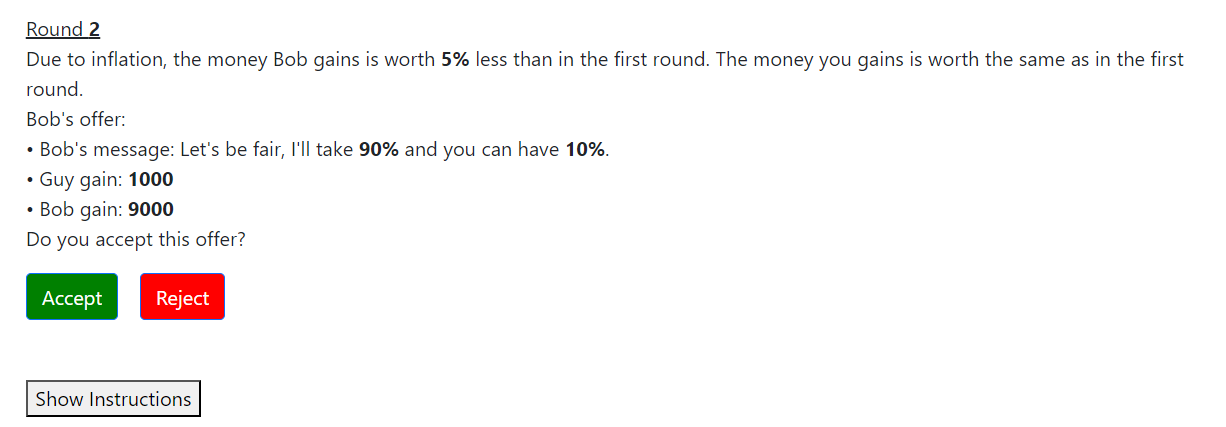
\includegraphics[width=0.9\textwidth,height=\textheight,keepaspectratio]{screenshots/bargaining_receiver.png}}
\caption{An example of a decision screen shown to a human player during his second turn in a Bargaining game.}
\label{fig:bargaining_receiver}
\end{figure}

\begin{figure}[H]
\raggedright
\centering
\fbox{
\includegraphics[width=0.3\textwidth,keepaspectratio]{screenshots/bargaining_response.png}}
\caption{An example of a response screen shown to human players during his second turn in a Bargaining game.}
\label{fig:bargaining_response}
\end{figure}


\subsubsection{Negotiation Games Screenshots}

\begin{figure}[H]
\centering
\fbox{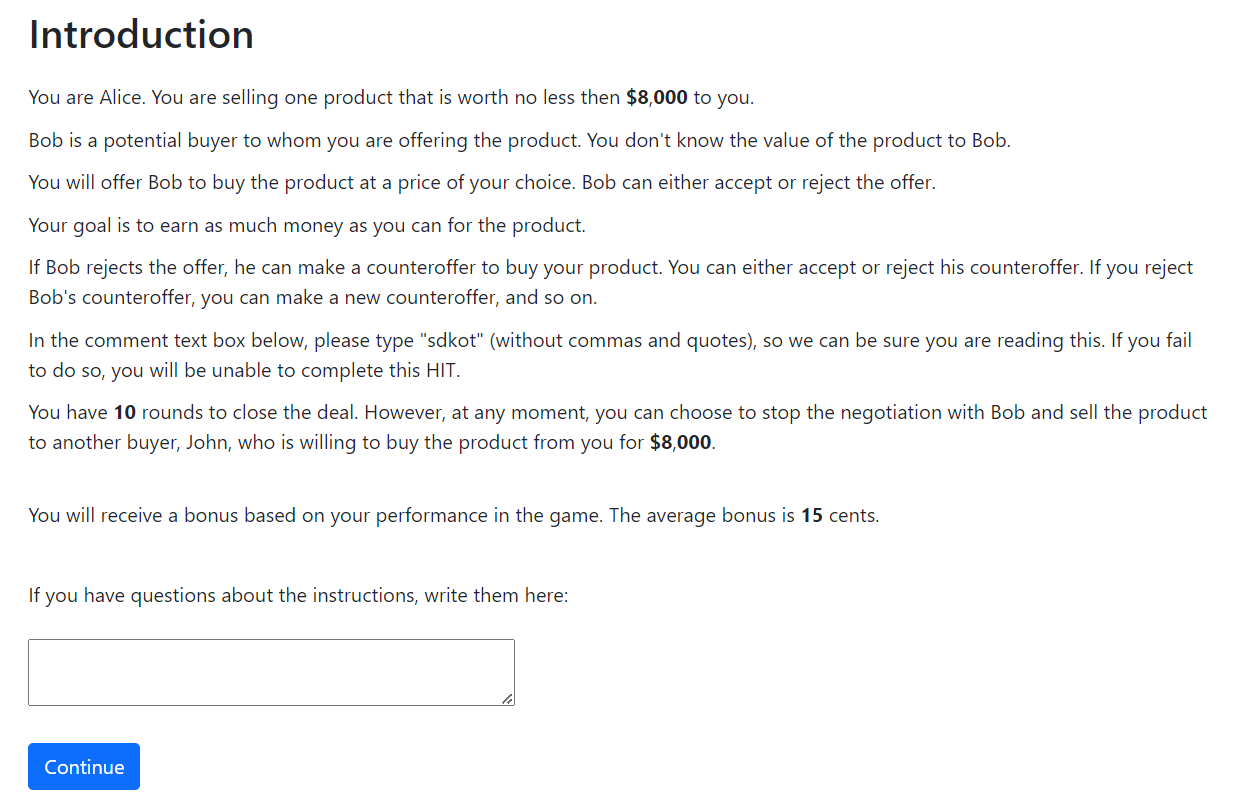
\includegraphics[width=0.8\textwidth,height=\textheight,keepaspectratio]{screenshots/negotiation_intro.png}}
\caption{An example of an instruction screen shown to a human sellers at the start of a Negotiation game.}
\label{fig:negotiation_intro}
\end{figure}

\begin{figure}[H]
\centering
\fbox{
\includegraphics[width=0.8\textwidth,height=\textheight,keepaspectratio]{screenshots/negotiation_proposer.png}}
\caption{An example of a proposition screen shown to human sellers during his first turn in a Negotiation game.}
\label{fig:negotiation_proposer}
\end{figure}

\begin{figure}[H]
\centering
\fbox{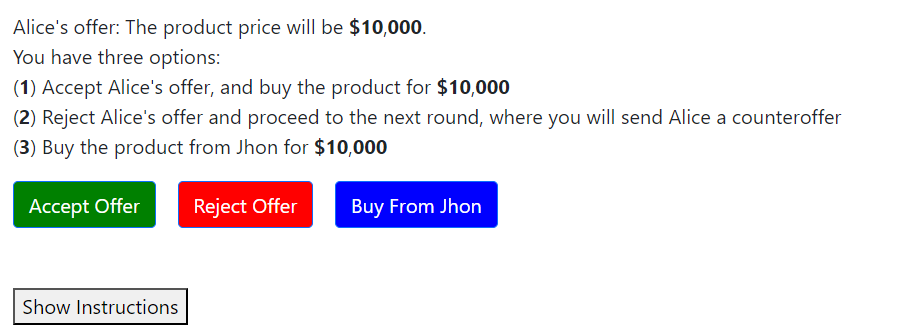
\includegraphics[width=0.8\textwidth,height=\textheight,keepaspectratio]{screenshots/negotiation_receiver.png}}
\caption{An example of a decision screen shown to human buyers during his first turn in a Negotiation game.}
\label{fig:negotiation_receiver}
\end{figure}

\begin{figure}[H]
\centering
\fbox{
\includegraphics[width=0.8\textwidth,height=\textheight,keepaspectratio]{screenshots/final_quiz.png}}
\caption{An example of a final quiz screen shown to human sellers at the end of a Negotiation game.}
\label{fig:fina_quiz}
\end{figure}

\subsubsection{Persuasion Games Screenshots}

\begin{figure}[H]
\centering
\fbox{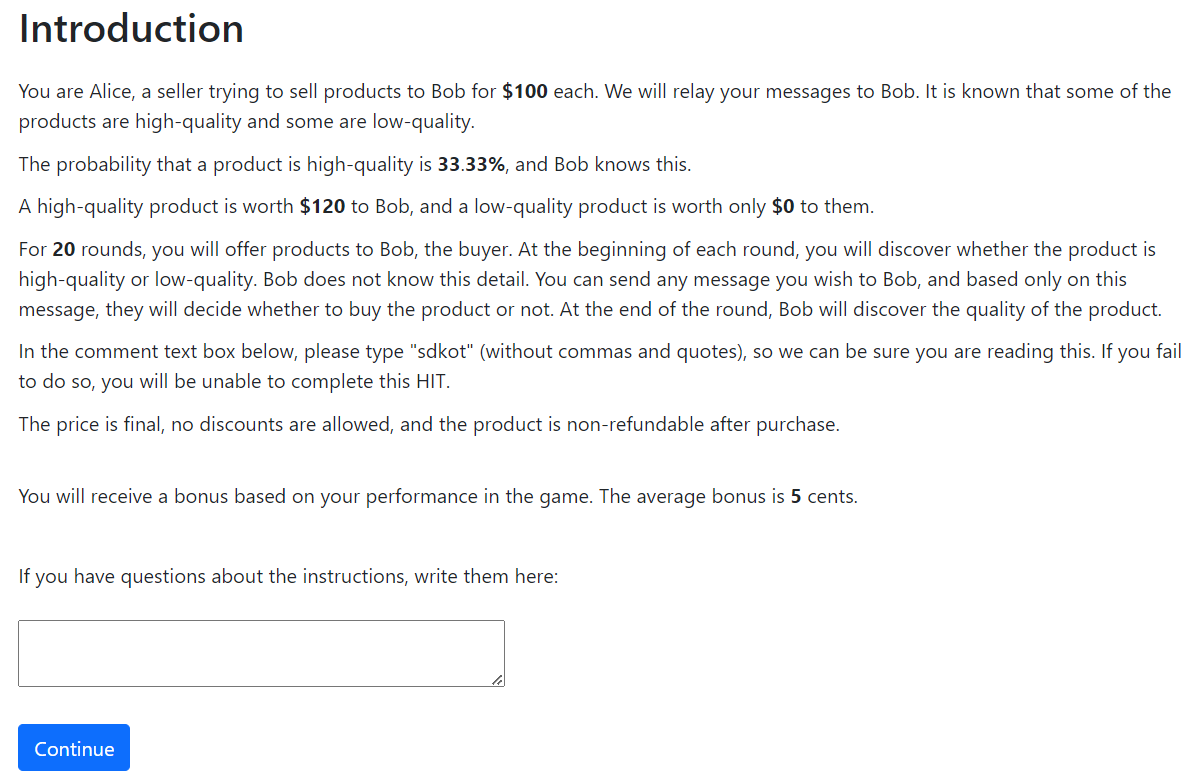
\includegraphics[width=0.8\textwidth,height=\textheight,keepaspectratio]{screenshots/persuasion_seller_intro.png}}
\caption{An example of an instruction screen shown to human sellers at the start of a Persuasion game.}
\label{fig:persuasion_seller_intro}
\end{figure}

\begin{figure}[H]
\centering
\fbox{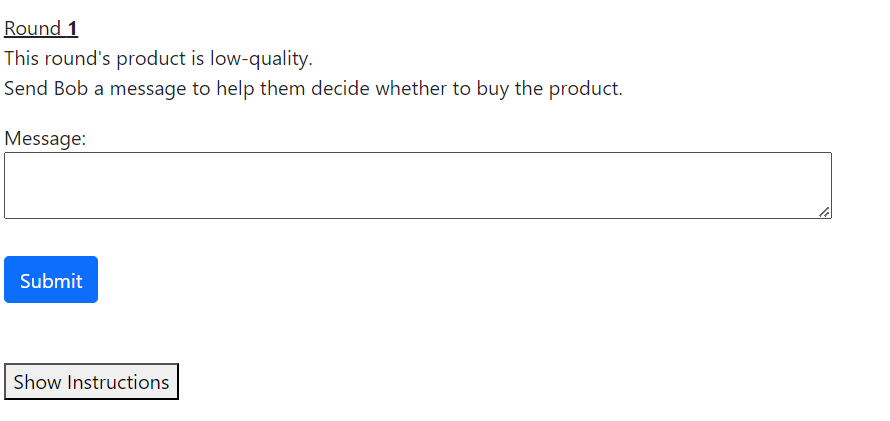
\includegraphics[width=0.8\textwidth,height=\textheight,keepaspectratio]{screenshots/persuasion_proposer.png}}
\caption{An example of a proposition screen shown to human sellers during his first turn in a Persuasion game.}
\label{fig:persuasion_proposer}
\end{figure}

\begin{figure}[H]
\centering
\fbox{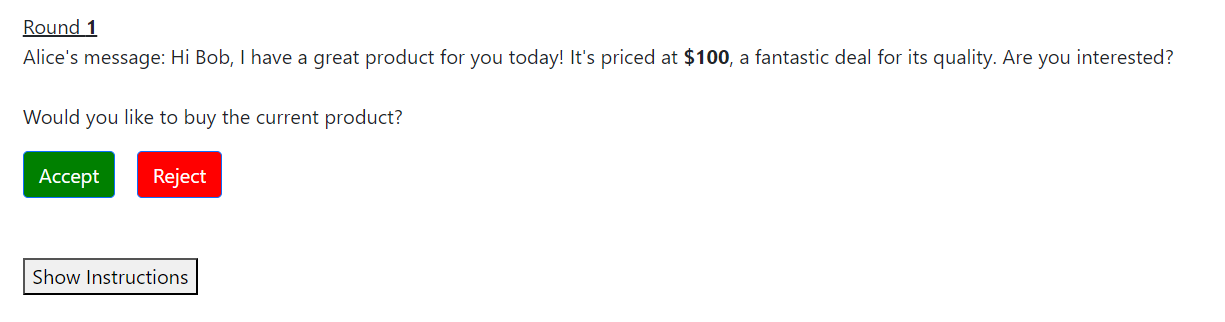
\includegraphics[width=0.8\textwidth,height=\textheight,keepaspectratio]{screenshots/persuasion_receiver.png}}
\caption{An example of a decision screen shown to human buyers during his first turn in a Persuasion game.}
\label{fig:persuasion_receiver}
\end{figure}

\begin{figure}[H]
\centering
\fbox{
\includegraphics[width=0.8\textwidth,height=\textheight,keepaspectratio]{screenshots/game_over.png}}
\caption{An example of a game over screen shown to human players at the end of a Persuasion game.}
\label{fig:game_over}
\end{figure}

\subsection{Selection of Configurations for Human Data Collection}
\label{app:human_configs}
In this appendix, we describe the method used to select which configurations human players would play and how many times each configuration would be played. Each configuration is defined by both the game parameters and the role of the human player (Alice or Bob).

For each family of games, we arbitrarily defined one configuration, which we referred to as the \textit{main configuration}. This configuration contains the parameters that we deemed most interesting. For every main configuration, we collected data for both possible roles of the human player (Alice or Bob). In persuasion games, we defined two main configurations: one for recurring buyers and one for manipulated buyers, due to the significant theoretical differences arising from this parameter. We collected the largest amount of data from the main configurations to allow for more in-depth follow-up research.

Configurations that were identical to one of the main configurations except for one parameter\footnote{In bargaining games, we defined a change in both players' discount factors as a change in one parameter} were called \textit{variants of the main configuration}. We collected data for all of these configurations as well.

Additionally, we randomly sampled 5\% of the other configurations and collected data from them as well. These configurations were referred to as \textit{random configurations}.

Due to the desire to allocate the data collection budget to complex games, we did not collect any data from games in which the human player was required to play at most one round (single-round bargaining games and persuasion games in which the human player is a manipulated buyer).

For each category, we determined the number of games we wanted to collect from each configuration belonging to it. This decision was made based on budgetary considerations. In persuasion games, we were able to collect fewer games from each configuration due to the fact that these games take longer to complete (and therefore, the payment players received for participating in them was higher). Table \ref{tab:human_data_config} describes the number of configurations that belonged to each category for each game and the minimum number of games we collected from each category.\footnote{Since the games were played in parallel, for some configurations we collected more games than required. For 113 configurations, we collected one more game than required; for 4 configurations, we collected 2 more games than required; and for one configuration, we collected 3 more games than required.}

\begin{table}[h]
    \centering
        \caption{The number of configurations belonging to each category for each game family, as well as the number of human players who played each configuration within each category.}

    \begin{tabular}{c|cc|cc|cc}
    \toprule
     & \multicolumn{2}{|c}{Bargaining} & \multicolumn{2}{|c}{Negotiation} & \multicolumn{2}{|c}{Persuasion} \\
     Type & \# config. & \# games & \# config. & \# games & \# config. & \# games \\
    \midrule
    main & 2 & 50 & 2 & 50 & 3 & 30 \\
    variant & 40 & 25 & 22 & 25 & 30 & 8 \\
    random & 36 & 15 & 36 & 15 & 24 & 5 \\
    \bottomrule
    \end{tabular}
    \label{tab:human_data_config}
\end{table}


\subsection{Attention Checks for Human Players}
\label{app:attention_test}
In this appendix, we describe the two attention tests that human players were required to complete. The purpose of these tests was to ensure that the human players stayed focused on the game and made conscious decisions, rather than random choices to finish the game as quickly as possible. The players were aware that their attention would be tested during the game, and they knew that they would not be paid for the task if they failed these tests. Out of the 4,652 players who started the game, 1,247 players (representing 26.8\% of those who began the game) failed one of the tests and were not included in the final dataset.

The first test appeared on the instruction screen. Toward the end of the instructions, a line requested players to write the code word "sdkot" in a text box that appeared at the end of the instructions phase. Players who did not write this word were immediately disqualified and did not start the game, as they did not carefully read the instructions. A total of 412 players, representing 8.9\% of those who began the game, failed this test.

The second test appeared at the end of the game. The human players were asked a basic question that depended on the family of the game they played. They were required to select the correct answer from four possible options. Players who participated in a bargaining game were asked about the inflation rate in their game (499 players, representing 22.7\% of respondents, failed this question and were excluded from the dataset). Players who participated in a negotiation game were asked about the value of the product for them (68 players, representing 12.3\% of respondents, failed this question and were excluded from the dataset). Players who participated in a persuasion game were asked about the price of products in the game (268 players, representing 18\% of respondents, failed this question and were excluded from the dataset). In total, 835 players, representing 19.7\% of respondents, failed the final question and were excluded from the dataset.
